\documentclass[11pt]{jsarticle}  % 文字の大きさは調整可能
%紙サイズ：A4(297mm×210mm)
%文字サイズ：11pt(調整可能)

\usepackage{zemistyle}
%\usepackage{amsmath}
%\usepackage{amsfonts}
%\usepackage{enumerate}
\usepackage{amssymb}
\usepackage{booktabs}
\usepackage{subcaption}
\usepackage{multirow}
\usepackage{newtxtext,newtxmath}%英数字書体として「Times new Roman」を使う
\usepackage[dvipdfmx]{graphicx}
\usepackage[hyphens]{url}

\setcounter{topnumber}{6}
\setcounter{bottomnumber}{5}
\setcounter{totalnumber}{11}
\setcounter{dbltopnumber}{5}
\renewcommand{\topfraction}{.999}
\renewcommand{\dbltopfraction}{.999}
\renewcommand{\bottomfraction}{.999}
\renewcommand{\textfraction}{.001}
\renewcommand{\floatpagefraction}{.999}
\renewcommand{\dblfloatpagefraction}{.999}
\renewcommand{\baselinestretch}{1.0} % 行間の調整
\newcommand{\Hline}{\noalign{\hrule height 0.4mm}}
\newcommand{\vect}[1]{\mbox{\boldmath$#1$}}
\newcommand{\svect}[1]{\mbox{\scriptsize\boldmath $#1$}}


\begin{document}
%%%%%%%%%%%%%%%%%%%%%%%%%%%%%%%%%%%%%%%%%%%%%%%%%%%%%%%%%%%%%%%%%%%%%%%%%%%%%%%%%%%%%%%%%%%%%%
% Title and author information
%%%%%%%%%%%%%%%%%%%%%%%%%%%%%%%%%%%%%%%%%%%%%%%%%%%%%%%%%%%%%%%%%%%%%%%%%%%%%%%%%%%%%%%%%%%%%%
\title{
クラス情報による誘導が可能な Discrete Flow Matching による\\データ生成モデルの検討}

\date{\large \today}
\author{
  \large 24559 ~ 藤岡 雅大
}

\maketitle
%%%%%%%%%%%%%%%%%%%%%%%%%%%%%%%%%%%%%%%%%%%%%%%%%%%%%%%%%%%%%%%%%%%%%%%
% Beginning of the document
%%%%%%%%%%%%%%%%%%%%%%%%%%%%%%%%%%%%%%%%%%%%%%%%%%%%%%%%%%%%%%%%%%%
\section{はじめに}
Discrete Flow Matching\cite{DFM} (DFM)は，
連続空間において常微分方程式により生成過程を定義するFlow Matching\cite{FMGM} (FM) を離散空間へと拡張した手法である．
DFMは，連続時間マルコフ過程における確率経路の回帰を通じて離散データを生成する，非自己回帰型生成モデルの枠組みであり，
言語生成や画像生成といった高次元離散データの評価タスクにおいて高い性能を示している．

生成モデルにおいて出力を制御することは，生成モデルの応用範囲を広げるだけでなく，ユーザの意図に沿った出力を得るために不可欠である．
しかし，現行のDFMでは，言語翻訳のような状態初期値と出力の対応付けによる条件付け手法は存在するが，
クラス情報などの状態以外の入力によって生成結果を誘導する手法が未確立である．

一方，Discrete Diffusion Models\cite{DDM} (DDM) は，離散時間のマルコフ過程を通じてノイズを付与した離散データの
逆過程を学習する手法であり，
この手法の出力制御方法として，クラス情報を用いるClassifier-Free Guidance\cite{CFDDM} (CFDDM) が提案されている．

本研究では，Classifier-Free GuidanceをDFMに適用し，DFMを用いたクラス情報による出力誘導の定式化について検討する．
また，提案手法の有効性を確認するために画像生成実験を実施し，
生成画像に含まれるクラス情報の妥当性をFréchet Inception Distance\cite{FID}（FID）
およびクラス分類モデルを用いたダイバージェンスによって評価した．


%%%%%%%%%%%%%%%%%%%%%%%%%%%%%%%%%%%%%%%%%%%%%%%%%%%%%%%%%%%%%%%%%%%
\section{Discrete Flow Matching\cite{DFM}}
\label{sec:dfm}
Discrete Flow Matching (DFM) は，連続空間のFlow Matching (FM) の枠組みを離散データ生成に適応した手法であり，
離散空間上での非自己回帰型生成モデルフレームワークの一種である．

ここでは，離散空間$\mathcal{D}$を$K$通りの離散値を持つ$d$次元のデータ空間$\{K\}^d$とし，
$X_t \in \mathcal{D}$を時刻$t \in [0, 1]$における確率変数とする．
DFMは，ソース分布$p$から得られるソースサンプル$X_0 \sim p$から，
ターゲット分布$q$に従うターゲットサンプル$X_1 \sim q$を生成することを目的とする．
そのために，$p$と$q$を結ぶ確率経路$p_t$を定義し，その経路に沿った確率質量関数の時間発展を連続時間マルコフ過程 (CTMC) の形式でモデル化する．
具体的には，時刻$t$での確率変数$X_t$が与えられたとき，時刻$t+h$の確率変数$X_{t+h}$は0から$d$までの各トークン次元$i \in \{d\}$ごとに独立に次のようにサンプリングされる．
\begin{equation}
  X_{t+h}^{(i)} \sim \delta_{X_t^{(i)}}(\cdot) + h u_t^{(i)}(\cdot, X_t) \notag
\end{equation}
ここで，$u_t^{(i)}(\cdot, X_t)$は時刻$t$における状態$X_t$が与えられたときの次元$i$におけるベクトル場であり，$\delta_x(\cdot)$はDiracのデルタ関数である．

%%%%%%%%%%%%%%%%%%%%%%%%%%%%%%%%%%
\subsection{DFMの学習}
\label{sec:dfm_learning}
DFMの学習は，各時刻$t$における$u_t^{(i)}(\cdot, X_t)$を回帰することで行われる．
機械学習モデルの損失関数$\mathcal{L}$は，CTMCにより決定される$u_t^{(i)}(\cdot,X_t)$と，
$X_t$が与えられたときのモデル出力$\hat{u_t}^{(i)}(\cdot, X_t; \theta)$とのBregmanダイバージェンス$D(\cdot, \cdot)$の，次元$i$ごとの和の期待値で表される\cite{FMGuide}．
\begin{equation}
  \label{eq:dfm_loss}
  \mathcal{L}(\theta) = 
  \mathbb{E}_{t, X_t}\left[\sum_{i \in \{d\}} D_{X_t}\left(u_t^{(i)}(\cdot, X_t) , \hat{u_t}^{(i)}(\cdot, X_t; \theta)\right)\right]
\end{equation}
また，任意の状態空間$\mathcal{Z}$から得られる確率変数$Z$で条件付けた条件付きベクトル場$u_t^{(i)}(\cdot, X_t \mid Z)$とモデル出力とのBregmanダイバージェンス
で定義される損失関数と，式(\ref{eq:dfm_loss})の損失関数は，モデルパラメータ$\theta$の勾配が一致することが知られている\cite{FMGuide}．
\begin{equation}
  \nabla_\theta\mathcal{L}(\theta) = 
  \nabla_\theta \mathbb{E}_{t, X_t, Z}\left[\sum_{i \in \{d\}} D_{X_t}\left(u_t^{(i)}(\cdot, X_t \mid Z) , \hat{u_t}^{(i)}(\cdot, X_t; \theta)\right)\right] \notag
\end{equation}
そのため，実装上では$Z$をソースデータ$x_0$とターゲットデータ$x_1$とした条件付きベクトル場$u_t^{(i)}(\cdot, X_t \mid x_0, x_1)$を
用いて損失関数を定義する．


%%%%%%%%%%%%%%%%%%%%%%%%%%%%%%%%%%%%%%%%%%%%%%%%%%%%%%%%%%%%%%%%%%%
\section{Classifier-Free Discrete Diffusion Models\cite{CFDDM}}
\label{sec:cfg_discrete}
Discrete Diffusion Models (DDM)\cite{DDM}は，Diffusion Models (DM)\cite{DM}を離散データに適用したモデルフレームワークである．
DFMと異なり，離散時間のマルコフ過程によるノイズデータ汚染のデノイジングを学習することでデータ生成を行う．

%%%%%%%%%%%%%%%%%%%%%%%%%%%%%%%%%%
\subsection{DDMにおけるClassifier-Free Guidance}
DDMでは，クラス条件制御を行う手法としてClassifier-Free Guidance\cite{CFDDM}が提案されている．
$x_t \in \mathcal{D} = \{K\}^d$を離散時刻$t \in \{T\}$における状態変数とし，$c\in \mathcal{C}$を状態空間$C$内の条件変数とする．
DDMでのClassifier-Free Guidanceでは，状態変数$x_{t+1}$の事後分布を，
条件付き事後分布$p_{t+1 \mid \mathcal{C}, t}(x_{t+1} \mid c,x_{t})$と
非条件付き事後分布$p_{t+1 \mid t}(x_{t+1} \mid x_{t})$を用いて，各次元$i \in \{d\}$ごと独立に定義する．
\begin{align}
  \label{eq:ddm_cfg}
  &p_{\gamma, t+1 \mid \mathcal{C}, t}(x_{t+1} \mid c,x_{t}) \notag \\
  = &\prod_{i=1}^d
    \frac{p_{t+1 \mid \mathcal{C}, t}(x_{t+1}^{(i)} \mid c,x_{t})^\gamma
      p_{t+1 \mid t}(x_{t+1}^{(i)} \mid x_{t})^{1-\gamma}}
    {\sum_{x_{t+1}'} p_{t+1 \mid \mathcal{C}, t}(x_{t+1}' \mid c,x_{t})^\gamma
    p_{t+1 \mid t}(x_{t+1}' \mid x_{t})^{1-\gamma}} \notag
\end{align}
なお，$\gamma$は$x_{t+1}$の$c$に対する尤度を調節する温度パラメータであり，出力分布の条件忠実性と多様性のトレードオフを調節することができる．

ここで，マスクされた条件変数を入力としたモデル出力を非条件付き生成とみなすことで，
条件付き生成と非条件付き生成において同一のモデルパラメータ$\theta$を用いることができる．
なお，一般的に学習時には，条件変数をバッチ単位で一定の確率でマスクする．

また，DDMでは離散時間間隔を0に近づける極限において，データ汚染過程のマルコフ過程がCTMCに収束することが知られている．
この点で，DFMとDDMは共通の枠組みに属し，DDMで提案されたClassifier-Free GuidanceのDFMへの適用が期待できる．
%%%%%%%%%%%%%%%%%%%%%%%%%%%%%%%%%%%%%%%%%%%%%%%%%%%%%%%%%%%%%%%%%%%


\section{DFMにおける出力の条件付け}
\label{sec:cdfm}
提案手法では，任意の状態空間$\mathcal{C}$内の条件変数 $c \in \mathcal{C}$でDFMの条件付けを行う．
具体的には，時刻$t \in [0, 1]$で$c$と状態変数$x \in \mathcal{D}$が与えられたとき，
条件付き確率経路$p_{t+h \mid \mathcal{C}, t}(y \mid x, c)$を時刻$t+h$で状態変数$y \in \mathcal{D}$に遷移する条件付き確率経路とし，
ベクトル場$u_{t \mid \mathcal{C}}(y, x \mid c)$を時刻$t+h$で$x$から$y$への遷移を表す条件付きベクトル場とする．
このとき，条件付けられたDFM (CDFM) における$p_{t+h \mid \mathcal{C}, t}(y \mid x, c)$は
$u_{t \mid \mathcal{C}}(y, x \mid c)$を用いて次式で表される．
\begin{equation}
  \label{eq:dfm_transition_porb_cond}
  p_{t+h \mid \mathcal{C}, t}(y \mid c, x) = \delta_x(y) + h u_{t \mid \mathcal{C}}(y, x \mid c)
\end{equation}
また，DFMと同様に各トークン次元$i \in \{d\}$ごとに独立にサンプリングされると仮定する．
\begin{align}
  X_{t+h}^{(i)} &\sim p_{t+h \mid \mathcal{C}, t}^{(i)}(y \mid c, x) \notag \\
    &= \delta_{X_t^{(i)}}(\cdot) + h u_{t \mid \mathcal{C}}^{(i)}(\cdot, X_t \mid c) \notag
\end{align}
また，損失関数は$c$を用いて以下のように書き換えられる．
\begin{equation}
  \mathcal{L}(\theta) = 
    \mathbb{E}_{t, X_t, Z, c}\left[ \sum_{i \in \{d\}}
      D_{X_t}\left(
        u_{t \mid \mathcal{C}}^{(i)}(\cdot, X_t \mid Z, c) , 
        \hat{u}_{t \mid \mathcal{C}}^{(i)}(\cdot, X_t \mid c; \theta)\right)\right] \notag
\end{equation}
%%%%%%%%%%%%%%%%%%%%%%%%%%%%%%%%%%%%%%%%%%%%%%%%%%%%%%%%%%%%%%%%%%%


\section{CDFMにおけるClassifier-Free Guidance}
提案手法として，
DDMでのClassifier-Free GuidanceをDFMに適用し，
CDFMによるモデル出力が条件変数に対する尤度を高くするように誘導する手法を提案する．

%%%%%%%%%%%%%%%%%%%%%%%%%%%%%%%%%%
\subsection{CDFMにおけるClassifier-Free Guidanceの導出},
式(\ref{eq:dfm_transition_porb_cond})の条件付き確率経路$p_{t+h \mid \mathcal{C}, t}(y \mid c, x)$は
ベイズの定理を用いて次のように表される．
\begin{equation}
  \label{eq:dfm_transition_porb_cond_bayes}
  p_{t+h \mid \mathcal{C}, t}(y \mid c, x) = \frac{p_{\mathcal{C} \mid t+h, t}(c \mid y, x)p_{t+h \mid t}(y \mid x)}{p_{\mathcal{C} \mid t}(c \mid x)} 
\end{equation}
式(\ref{eq:dfm_transition_porb_cond_bayes})の変形を踏まえ，
温度パラメータ$\gamma \in \mathbb{R}$を用いて誘導補正した条件付き補正確率経路$p_{\gamma, t+h \mid \mathcal{C}, t}$を以下のように定義する．
\begin{align}
  \label{eq:conditional_transition_prob_gamma}
  p_{\gamma, t+h \mid \mathcal{C}, t}&(y \mid c, x)
  = \frac{\frac{p_{\mathcal{C} \mid t+h, t}(c \mid y, x)^\gamma p_{t+h \mid t}(y \mid x)}{p_{\mathcal{C} \mid t}(c \mid x)}}{\sum_{y'} \frac{p_{\mathcal{C} \mid t+h, t}(c \mid y', x)^\gamma p_{t+h \mid t}(y' \mid x)}{p_{\mathcal{C} \mid t}(c \mid x)}}
\end{align}
式(\ref{eq:conditional_transition_prob_gamma})は，ベイズの定理を用いて次のように変形できる．
\begin{equation}
  \label{eq:conditional_transition_prob_gamma_bayes}
  p_{\gamma, t+h \mid \mathcal{C}, t}(y \mid c, x)
  = \frac
    {p_{t+h \mid \mathcal{C}, t}(y \mid c, x)^\gamma p_{t+h \mid t}(y \mid x)^{1-\gamma}}
    {\sum_{y'} p_{t+h \mid \mathcal{C}, t}(y' \mid c, x)^\gamma p_{t+h \mid t}(y' \mid x)^{1-\gamma}}
\end{equation}
式(\ref{eq:conditional_transition_prob_gamma_bayes})より，$p_{\gamma, t+h \mid \mathcal{C}, t}(y \mid c, x)$は，
DDMにおけるClassifier-Free Guidanceと同様に，
CDFMの条件付き確率経路$p_{t+h \mid \mathcal{C}, t}(y \mid c, x)$と
DFMの非条件付き確率経路$p_{t+h \mid t}(y \mid x)$を組み合わせた形となる．
また，$\gamma$はDDMにおけるClassifier-Free Guidanceと同様に$y$における$c$の尤度を調節するパラメータとして作用する．

また，$p_{t+h \mid \mathcal{C}, t}(y \mid c, x)$と$p_{t+h \mid t}(y \mid x)$は
それぞれ$y$のトークン次元$i \in \{d\}$ごとに独立であるため，
式(\ref{eq:conditional_transition_prob_gamma_bayes})は各トークン次元$i$ごとに分解できる．
\begin{equation}
  \label{eq:conditional_transition_prob_gamma_bayes_i}
  p_{\gamma, t+h \mid \mathcal{C}, t}(y^{(i)} \mid c, x)
    = \frac
    {p_{t+h \mid \mathcal{C}, t}(y^{(i)} \mid c, x)^\gamma p_{t+h \mid t}(y^{(i)} \mid x)^{1-\gamma}}
    {\sum_{y^{(i)}} p_{t+h \mid \mathcal{C}, t}(y^{(i)} \mid c, x)^\gamma p_{t+h \mid t}(y^{(i)} \mid x)^{1-\gamma}} \notag
\end{equation}

%%%%%%%%%%%%%%%%%%%%%%%%%%%%%%%%%%
\subsection{サンプリング方法}
サンプリング時には，学習済みCDFMとDFMを用いて十分大きい時間ステップ数$N$のオイラー近似によりサンプリングする．
各サンプリング時刻$t \in \{1/N, 2/N, ..., 1\}$において，
CDFMとDFMには同一の状態変数と条件変数を入力し，
それぞれのモデルから得られた出力から条件付き補正確率経路を算出する．
\begin{align}
  X_{t+h} &\sim p_{\gamma, t+h \mid \mathcal{C}, t}(\cdot \mid c, X_t) \notag
\end{align}

また，DDMでのClassifier-Free Guidanceと同様に，
マスクされた条件変数の入力に対応する出力をDFMの出力とすることで，
DFMとCDFMは同一のモデルを使用できる．
%%%%%%%%%%%%%%%%%%%%%%%%%%%%%%%%%%%%%%%%%%%%%%%%%%%%%%%%%%%%%%%%%%%


\section{実験}
提案手法のクラス情報による出力誘導効果を検証するため，
時刻ステップ数を1028とし，温度パラメータ$\gamma$を$\{0.0,~0.2,~0.5,~0.8,~1.0,~1.2,~1.5,~2.0,~3.0\}$の9通りで画像生成実験を行った．
実験では，離散値を持つデータセットとして，図\ref{fig:mnist_samples}のように画素値を固定閾値0.5で0と1に2値化したMNISTデータセット (Binarized MNIST) を用いた．
また，CDFMとDFM共通の機械学習モデルとしてU-Net\cite{UNet}(パラメータ数約113M)を実装した．
モデルの学習にはBinarized MNISTの学習データセットを用い，クラス情報としては画像ラベルと，
画像ラベルとは異なる特定のカテゴリを割り当てたマスクラベルを7:3の割合で入力して，
100エポックの学習を行った．
また，評価時には，Binarized MNISTの評価ラベルデータを用い，CDFMとDFMのクラス情報としてそれぞれ画像ラベルとマスクラベルを入力し，
画像生成を行った．

\begin{figure}[h]
  \centering
  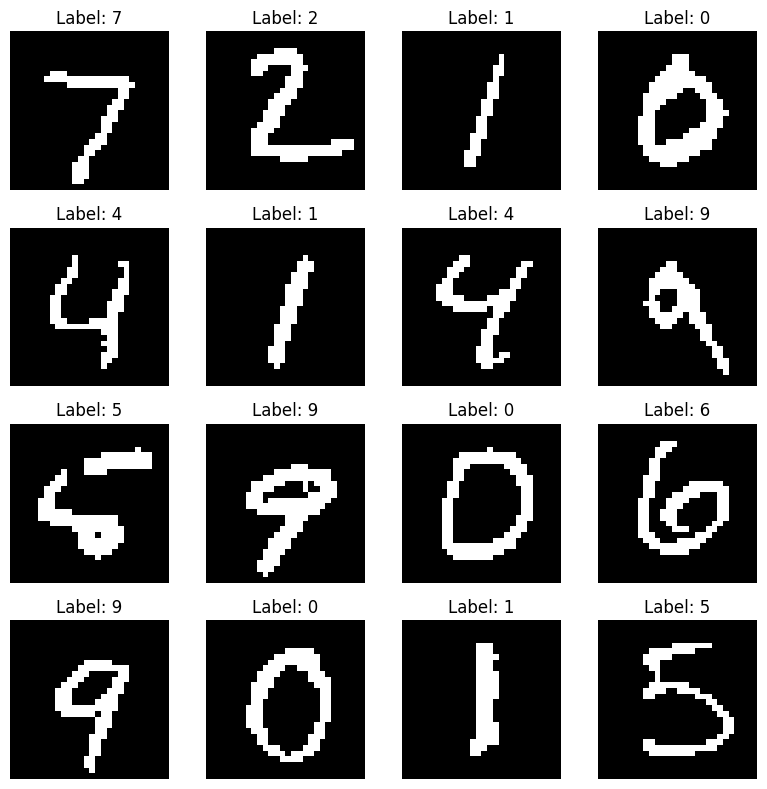
\includegraphics[width=0.3\linewidth]{figures/bmnist.png}  % 幅は画像に応じて調整
  \caption{閾値0.5のBinarized MNISTデータセット}
  \label{fig:mnist_samples}
\end{figure}

%%%%%%%%%%%%%%%%%%%%%%%%%%%%%%%%%%
\subsection{生成画像のFID評価}
\label{sec:fid}

\subsubsection{実験方法}
$\gamma$の各値に対して，生成画像群と評価データセットとの間でFID\cite{FID} (Fr\'echet Inception Distance) による評価を行った．
FIDは，クラスラベル別に計算したマクロ平均と，データセット全体の画像群に基づくマイクロ平均の2種類を算出した．
なお，FIDは生成画像群と実画像群の分布のFr\'echet距離を測る指標であり，値が小さいほど分布の類似度が高いことを示す．

\subsubsection{実験結果}
図 \ref{fig:fid_per_class} に$\gamma$の各値に対するクラスごとのFIDを，
図 \ref{fig:fid_macro_and_micro} にクラスごとのFIDのマイクロ平均とデータセット全体のマクロ平均を示す．

図 \ref{fig:fid_per_class} から，全てのクラスにおいて$\gamma=1.2$付近でFIDが最小を取る凸状の傾向が見られた．

また，図 \ref{fig:fid_macro_and_micro} から，$0 \leq \gamma \leq 0.5$の範囲では，
$\gamma$が小さいほどFIDのマクロ平均は大きくなる一方，FIDのマイクロ平均はマクロ平均ほどの増加は見られなかった．
これは，クラス条件付けのないDFMでは全クラスの分布を再現するように学習されるため，
$\gamma$によらずFIDのマイクロ平均は大幅な変化は見られない一方，
$\gamma$が0に近いほどクラス誘導の影響が小さくなり，生成画像と評価データセットのクラス分布が乖離していることを示唆している．
また，$1.2 \leq \gamma \leq 3.0$の範囲では，$\gamma$の増加に伴いFIDのマクロ平均とマイクロ平均ともに増加する傾向が見られた．
これは，$\gamma$が大きくなるほどクラス情報の影響が強くなり，
生成画像の分布がクラスに対して尤もらしい分布に偏ったことを示唆していると考えられる．

\begin{figure}[h]
  \centering
  \begin{minipage}[t]{0.48\linewidth}    % 幅を調整（0.48～0.49 が無難）
    \centering
    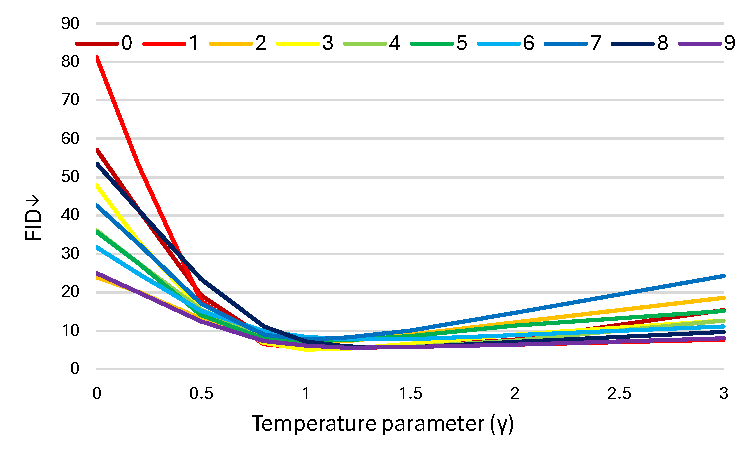
\includegraphics[width=\linewidth]{figures/fid_per_class.pdf}
    \caption{クラスラベル0〜9ごとのFID}
    \label{fig:fid_per_class}
  \end{minipage}
  \hfill                                % 図間の水平スペース
  \begin{minipage}[t]{0.48\linewidth}
    \centering
    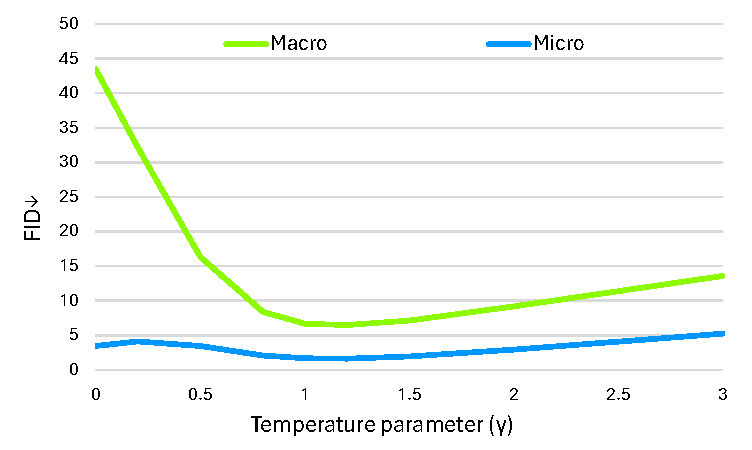
\includegraphics[width=\linewidth]{figures/fid_ave_all.pdf}
    \caption{クラスごとのFIDのマイクロ平均とマクロ平均}
    \label{fig:fid_macro_and_micro}
  \end{minipage}
\end{figure}


%%%%%%%%%%%%%%%%%%%%%%%%%%%%%%%%%%
\subsection{クラス分類結果のKLダイバージェンス評価}

\subsubsection{実験方法}
\ref{sec:fid}章で生成した画像を事前学習したクラス分類モデルに入力し，
出力されたクラス尤度と正解ラベルのone-hotベクトル間のKLダイバージェンスを，$\gamma$ごとに算出した．
クラス分類モデルにはWideResNet-28-10\cite{WRN}を用い，
Binarized MNISTの学習データセットを用いて100エポックの学習を行った．
また，クラス分類モデルの評価性能として，Binarized MNIST評価データセットに対する分類精度 (\%)および
正解ラベルとのKLダイバージェンスを表\ref{tbl:classifier_acc_kl}に示す．
\begin{table}[htbp]
  \centering
  % \small  % 必要に応じて
  \caption{ラベルごとの分類精度とKLダイバージェンス}
  \begin{tabular}{ccc}
    \hline
    Label & Accuracy (\%) & KL Divergence \\
    \hline
    0 & 99.90 & 0.23 $\times 10^{-2}$\\
    1 & 99.82 & 0.51 $\times 10^{-2}$\\
    2 & 99.61 & 0.60 $\times 10^{-2}$\\
    3 & 99.90 & 0.41 $\times 10^{-2}$\\
    4 & 99.49 & 2.56 $\times 10^{-2}$\\
    5 & 99.33 & 4.15 $\times 10^{-2}$\\
    6 & 99.16 & 3.23 $\times 10^{-2}$\\
    7 & 99.12 & 3.51 $\times 10^{-2}$\\
    8 & 99.69 & 0.76 $\times 10^{-2}$\\
    9 & 98.81 & 4.79 $\times 10^{-2}$\\
    \hline
    Average & 99.48 & 2.08 $\times 10^{-2}$\\
    \hline
  \end{tabular}
  \label{tbl:classifier_acc_kl}
\end{table}

\subsubsection{実験結果}
生成画像に対するクラス尤度と正解ラベルとのKLダイバージェンスのマクロ平均，
および表 \ref{tbl:classifier_acc_kl}に示す評価データセットに対するクラス尤度とのKLダイバージェンスのマクロ平均を，
$\gamma$ごとにプロットした結果を図 \ref{fig:kl_macro}に示す．
図 \ref{fig:kl_macro}より，$\gamma=0$から$\gamma=3.0$にかけてKLダイバージェンスのマクロ平均が単調に減少する様子が確認できた．
これは，$\gamma$の増加によりクラス情報の寄与が強まり，
生成画像のラベルに対する尤度が高まることを示唆していると考えられる．
また，$\gamma \geq 1.5$付近からは，生成画像のクラス分類によるKLダイバージェンスが，評価データセットのクラス分類による値を下回ることが確認できた．

\begin{figure}[h]
  \centering
  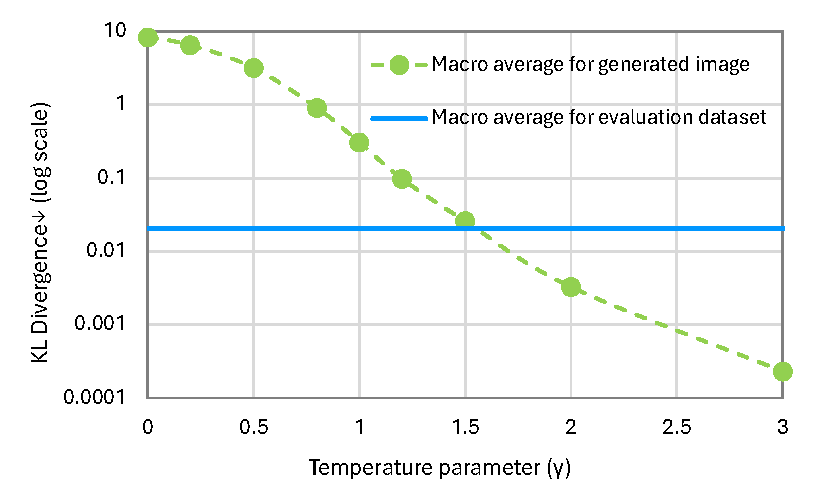
\includegraphics[width=0.6\linewidth]{figures/kl_ave.pdf}
  \caption{生成画像と評価データセットのKLダイバージェンス}
  \label{fig:kl_macro}
\end{figure}

%%%%%%%%%%%%%%%%%%%%%%%%%%%%%%%%%%
\subsection{定性評価}

\begin{figure*}[t]
  \centering
  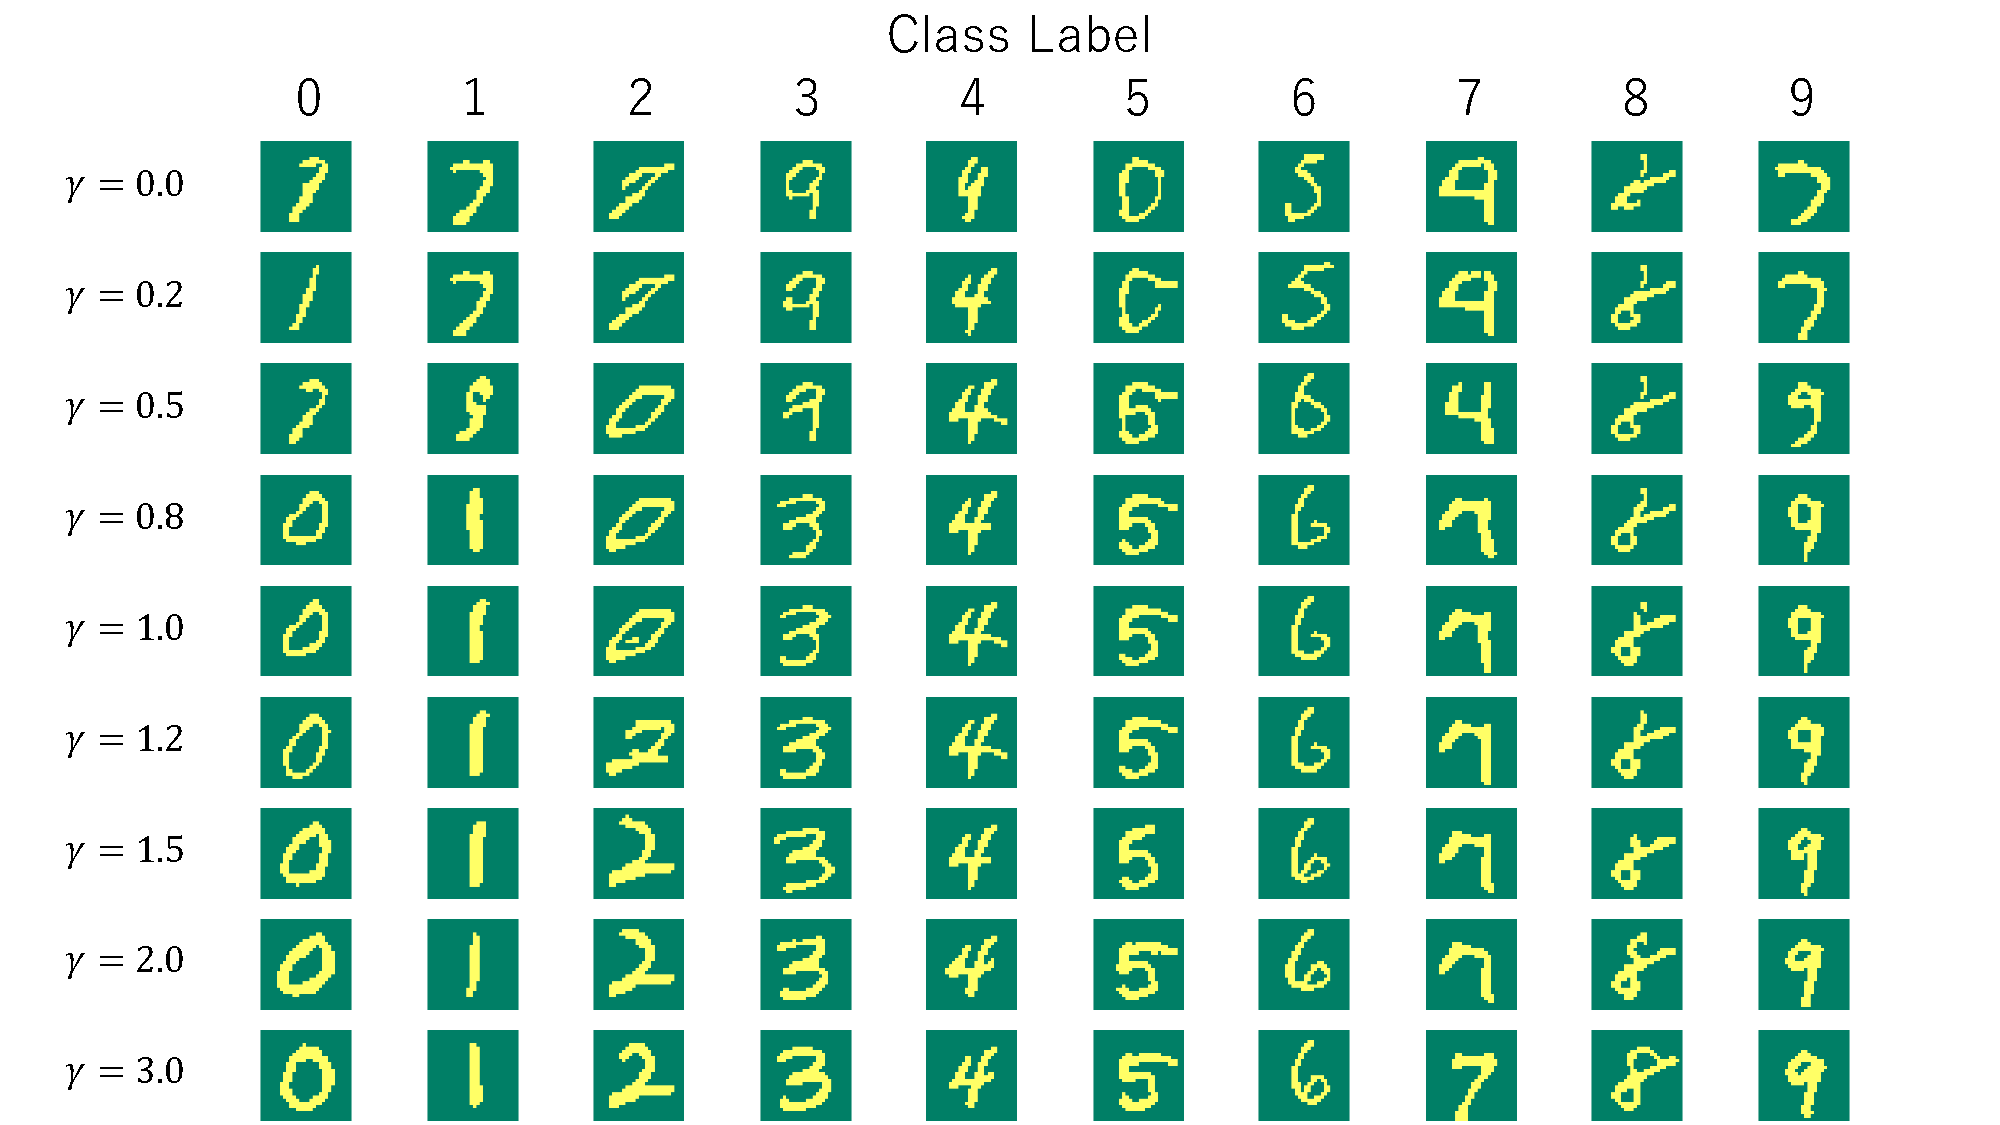
\includegraphics[height=0.3\textheight]{figures/qualitative.pdf}
  \caption{$\gamma$ごとの画像生成結果}
  \label{fig:qualitative_eval}
\end{figure*}

\subsubsection{実験方法}
$\gamma$ごとに共通の初期状態とクラス情報を与えて画像生成を行い，生成画像を定性的に比較した．
なお，付与する初期状態とクラス情報の組み合わせは，0から9の各クラスラベルごとの10通りで比較した．

\subsubsection{実験結果}
図 \ref{fig:qualitative_eval}に$\gamma$ごとの生成画像を示す．
DFMによる非条件付き生成である$\gamma=0.0$のときは，
クラス情報に依存しない画像が生成され，
複数の画像において複数のラベルの特徴が混在する様子が確認できた．
$\gamma=0.0$から1.0にかけては，生成画像が次第にクラス情報に対応する数字の形状へと近づいていく様子が確認できた．
一方，CDFMによる条件付き生成である$\gamma=1.0$において，
ラベル8やラベル2の生成画像ように，数字の形状が不明瞭であったりクラス情報と異なる数字が生成される例が確認できた．
しかし，$\gamma=1.0$から3.0にかけては，
全てのラベルの出力画像において，数字の形状がクラス情報と整合的な形状に近づいていく様子が確認できた．

%%%%%%%%%%%%%%%%%%%%%%%%%%%%%%%%%%%%%%%%%%%%%%%%%%%%%%%%%%%%%%%%%%%%%%%%%%%%%%%%%%%%%%%%
\section{おわりに}
本研究では，Discrete Flow Matchingにクラス情報を付与し，
サンプリング時において，クラス情報が出力へ与える影響を温度パラメータ$\gamma$を用いて調整する方法を定式化した．
評価データセットと生成画像のFIDの比較より，$\gamma$の値により出力画像の分布を誘導できることを確認した．
また，生成画像の分類器モデル出力とラベルとのKLダイバージェンスの比較と生成画像の定性評価より，
生成画像のラベルに対する尤もらしさを制御できるとも明らかにした．

今後の展望として，言語ドメインを始めとした画像以外の離散データでの評価や，
より自由度の高い条件付けの手法検討，
Guided Discrete Diffusion Modelとの性能，特性比較調査などが挙げられる．


\vspace{8ex}

%%%%%%%%%%%%%%%%%%%%%%%%%%%%%%%%%%%%%%%%%%%%%%%%%%%%%%%%%%%%%%%%%%%%%%%%%%%%%%%%%%%%%%%%
%\renewcommand{\baselinestretch}{0.9}
\newpage
\begin{thebibliography}{99}
\setlength{\itemsep}{1.5pt}
% \small % 必要に応じて

\bibitem{DFM}
I. Gat, T. Remez, N. Shaul, F. Kreuk, R. T. Q. Chen, G. Synnaeve, Y. Adi, and Y. Lipman,
``Discrete Flow Matching,''
Proc.\ 38th Conf.\ on Neural Information Processing Systems (NeurIPS 2024),
Dec.~2024.

\bibitem{FMGM}
Y. Lipman, R. T. Q. Chen, H. Ben-Hamu, M. Nickel, and M. Le,
``Flow Matching for Generative Modeling,''
Proc.\ 11th Int.\ Conf.\ on Learning Representations (ICLR 2023),
Apr.~2023.

\bibitem{DDM}
J. Austin, D. D. Johnson, J. Ho, D. Tarlow, and R. van den Berg,
``Structured Denoising Diffusion Models in Discrete State-Spaces,''
Proc.\ 35th Conf.\ on Neural Information Processing Systems (NeurIPS 2021),
pp.~17981--17993, Dec.~2021.

\bibitem{CFDDM}
Y. Schiff, S. S. Sahoo, H. Phung, G. Wang, S. Boshar, H. Dalla-torre, B. P. de Almeida, A. Rush, T. Pierrot, and V. Kuleshov,
``Simple Guidance Mechanisms for Discrete Diffusion Models,''
Proc.\ Causal and Object-Centric Representations for Robotics (CORR Workshop at CVPR 2024),
vol.~abs/2401.00001, Jun.~2024.

\bibitem{FID}
M. Heusel, H. Ramsauer, T. Unterthiner, B. Nessler, and S. Hochreiter,
``GANs Trained by a Two Time-Scale Update Rule Converge to a Local Nash Equilibrium,''
Proc.\ 31st Int.\ Conf.\ on Neural Information Processing Systems (NeurIPS 2017),
pp.~6626--6637, Dec.~2017.

\bibitem{FMGuide}
Y. Lipman, M. Havasi, P. Holderrieth, N. Shaul, M. Le, B. Karrer, R. T. Q. Chen, D. Lopez-Paz, H. Ben-Hamu, and I. Gat,
``Flow Matching Guide and Code,''
arXiv preprint arXiv:2412.06264, Dec.~2024.

\bibitem{DM}
J. Sohl-Dickstein, E. Weiss, N. Maheswaranathan, and S. Ganguli,
``Deep Unsupervised Learning using Nonequilibrium Thermodynamics,''
Proc.\ 32nd Int.\ Conf.\ on Machine Learning (ICML 2015),
pp.~2256--2265, Jul.~2015.

\bibitem{UNet}
O. Ronneberger, P. Fischer, and T. Brox,
``U-Net: Convolutional Networks for Biomedical Image Segmentation,''
in Lecture Notes in Computer Science, vol.\ 9351, 
Proc.\ 18th Int.\ Conf.\ on Medical Image Computing and Computer-Assisted Intervention (MICCAI 2015),
pp.~234--241, Sept.~2015.

\bibitem{WRN}
S. Zagoruyko and N. Komodakis,
``Wide Residual Networks,''
Proc.\ British Machine Vision Conf.\ (BMVC 2016),
Sept.~2016.

\end{thebibliography}

\end{document}